% Options for packages loaded elsewhere
\PassOptionsToPackage{unicode}{hyperref}
\PassOptionsToPackage{hyphens}{url}
%
\documentclass[
]{article}
\usepackage{amsmath,amssymb}
\usepackage{iftex}
\ifPDFTeX
  \usepackage[T1]{fontenc}
  \usepackage[utf8]{inputenc}
  \usepackage{textcomp} % provide euro and other symbols
\else % if luatex or xetex
  \usepackage{unicode-math} % this also loads fontspec
  \defaultfontfeatures{Scale=MatchLowercase}
  \defaultfontfeatures[\rmfamily]{Ligatures=TeX,Scale=1}
\fi
\usepackage{lmodern}
\ifPDFTeX\else
  % xetex/luatex font selection
\fi
% Use upquote if available, for straight quotes in verbatim environments
\IfFileExists{upquote.sty}{\usepackage{upquote}}{}
\IfFileExists{microtype.sty}{% use microtype if available
  \usepackage[]{microtype}
  \UseMicrotypeSet[protrusion]{basicmath} % disable protrusion for tt fonts
}{}
\makeatletter
\@ifundefined{KOMAClassName}{% if non-KOMA class
  \IfFileExists{parskip.sty}{%
    \usepackage{parskip}
  }{% else
    \setlength{\parindent}{0pt}
    \setlength{\parskip}{6pt plus 2pt minus 1pt}}
}{% if KOMA class
  \KOMAoptions{parskip=half}}
\makeatother
\usepackage{xcolor}
\usepackage[margin=1in]{geometry}
\usepackage{color}
\usepackage{fancyvrb}
\newcommand{\VerbBar}{|}
\newcommand{\VERB}{\Verb[commandchars=\\\{\}]}
\DefineVerbatimEnvironment{Highlighting}{Verbatim}{commandchars=\\\{\}}
% Add ',fontsize=\small' for more characters per line
\usepackage{framed}
\definecolor{shadecolor}{RGB}{248,248,248}
\newenvironment{Shaded}{\begin{snugshade}}{\end{snugshade}}
\newcommand{\AlertTok}[1]{\textcolor[rgb]{0.94,0.16,0.16}{#1}}
\newcommand{\AnnotationTok}[1]{\textcolor[rgb]{0.56,0.35,0.01}{\textbf{\textit{#1}}}}
\newcommand{\AttributeTok}[1]{\textcolor[rgb]{0.13,0.29,0.53}{#1}}
\newcommand{\BaseNTok}[1]{\textcolor[rgb]{0.00,0.00,0.81}{#1}}
\newcommand{\BuiltInTok}[1]{#1}
\newcommand{\CharTok}[1]{\textcolor[rgb]{0.31,0.60,0.02}{#1}}
\newcommand{\CommentTok}[1]{\textcolor[rgb]{0.56,0.35,0.01}{\textit{#1}}}
\newcommand{\CommentVarTok}[1]{\textcolor[rgb]{0.56,0.35,0.01}{\textbf{\textit{#1}}}}
\newcommand{\ConstantTok}[1]{\textcolor[rgb]{0.56,0.35,0.01}{#1}}
\newcommand{\ControlFlowTok}[1]{\textcolor[rgb]{0.13,0.29,0.53}{\textbf{#1}}}
\newcommand{\DataTypeTok}[1]{\textcolor[rgb]{0.13,0.29,0.53}{#1}}
\newcommand{\DecValTok}[1]{\textcolor[rgb]{0.00,0.00,0.81}{#1}}
\newcommand{\DocumentationTok}[1]{\textcolor[rgb]{0.56,0.35,0.01}{\textbf{\textit{#1}}}}
\newcommand{\ErrorTok}[1]{\textcolor[rgb]{0.64,0.00,0.00}{\textbf{#1}}}
\newcommand{\ExtensionTok}[1]{#1}
\newcommand{\FloatTok}[1]{\textcolor[rgb]{0.00,0.00,0.81}{#1}}
\newcommand{\FunctionTok}[1]{\textcolor[rgb]{0.13,0.29,0.53}{\textbf{#1}}}
\newcommand{\ImportTok}[1]{#1}
\newcommand{\InformationTok}[1]{\textcolor[rgb]{0.56,0.35,0.01}{\textbf{\textit{#1}}}}
\newcommand{\KeywordTok}[1]{\textcolor[rgb]{0.13,0.29,0.53}{\textbf{#1}}}
\newcommand{\NormalTok}[1]{#1}
\newcommand{\OperatorTok}[1]{\textcolor[rgb]{0.81,0.36,0.00}{\textbf{#1}}}
\newcommand{\OtherTok}[1]{\textcolor[rgb]{0.56,0.35,0.01}{#1}}
\newcommand{\PreprocessorTok}[1]{\textcolor[rgb]{0.56,0.35,0.01}{\textit{#1}}}
\newcommand{\RegionMarkerTok}[1]{#1}
\newcommand{\SpecialCharTok}[1]{\textcolor[rgb]{0.81,0.36,0.00}{\textbf{#1}}}
\newcommand{\SpecialStringTok}[1]{\textcolor[rgb]{0.31,0.60,0.02}{#1}}
\newcommand{\StringTok}[1]{\textcolor[rgb]{0.31,0.60,0.02}{#1}}
\newcommand{\VariableTok}[1]{\textcolor[rgb]{0.00,0.00,0.00}{#1}}
\newcommand{\VerbatimStringTok}[1]{\textcolor[rgb]{0.31,0.60,0.02}{#1}}
\newcommand{\WarningTok}[1]{\textcolor[rgb]{0.56,0.35,0.01}{\textbf{\textit{#1}}}}
\usepackage{graphicx}
\makeatletter
\def\maxwidth{\ifdim\Gin@nat@width>\linewidth\linewidth\else\Gin@nat@width\fi}
\def\maxheight{\ifdim\Gin@nat@height>\textheight\textheight\else\Gin@nat@height\fi}
\makeatother
% Scale images if necessary, so that they will not overflow the page
% margins by default, and it is still possible to overwrite the defaults
% using explicit options in \includegraphics[width, height, ...]{}
\setkeys{Gin}{width=\maxwidth,height=\maxheight,keepaspectratio}
% Set default figure placement to htbp
\makeatletter
\def\fps@figure{htbp}
\makeatother
\setlength{\emergencystretch}{3em} % prevent overfull lines
\providecommand{\tightlist}{%
  \setlength{\itemsep}{0pt}\setlength{\parskip}{0pt}}
\setcounter{secnumdepth}{-\maxdimen} % remove section numbering
\ifLuaTeX
  \usepackage{selnolig}  % disable illegal ligatures
\fi
\usepackage{bookmark}
\IfFileExists{xurl.sty}{\usepackage{xurl}}{} % add URL line breaks if available
\urlstyle{same}
\hypersetup{
  pdftitle={Data Wrangling with tidyr},
  hidelinks,
  pdfcreator={LaTeX via pandoc}}

\title{Data Wrangling with tidyr}
\author{}
\date{\vspace{-2.5em}}

\begin{document}
\maketitle

\begin{itemize}
\tightlist
\item
  Describe the concept of a wide and a long table format and for which
  purpose those formats are useful.
\item
  Describe the roles of variable names and their associated values when
  a table is reshaped.
\item
  Reshape a dataframe from long to wide format and back with the
  \texttt{pivot\_wider} and \texttt{pivot\_longer} commands from the
  \textbf{\texttt{tidyr}} package.
\item
  Export a dataframe to a csv file.
\end{itemize}

\begin{itemize}
\tightlist
\item
  How can I reformat a data frame to meet my needs?
\end{itemize}

\textbf{\texttt{dplyr}} pairs nicely with \textbf{\texttt{tidyr}} which
enables you to swiftly convert between different data formats (long
vs.~wide) for plotting and analysis. To learn more about
\textbf{\texttt{tidyr}} after the workshop, you may want to check out
this
\href{https://raw.githubusercontent.com/rstudio/cheatsheets/main/tidyr.pdf}{handy
data tidying with \textbf{\texttt{tidyr}} cheatsheet}.

To make sure everyone will use the same dataset for this lesson, we'll
read again the SAFI dataset that we downloaded earlier.

\begin{Shaded}
\begin{Highlighting}[]
\DocumentationTok{\#\# load the tidyverse}
\FunctionTok{library}\NormalTok{(tidyverse)}
\FunctionTok{library}\NormalTok{(here)}

\NormalTok{interviews }\OtherTok{\textless{}{-}} \FunctionTok{read\_csv}\NormalTok{(}\FunctionTok{here}\NormalTok{(}\StringTok{"data"}\NormalTok{, }\StringTok{"SAFI\_clean.csv"}\NormalTok{), }\AttributeTok{na =} \StringTok{"NULL"}\NormalTok{)}

\DocumentationTok{\#\# inspect the data}
\NormalTok{interviews}

\DocumentationTok{\#\# preview the data}
\CommentTok{\# view(interviews)}
\end{Highlighting}
\end{Shaded}

\subsection{Reshaping with pivot\_wider() and
pivot\_longer()}\label{reshaping-with-pivot_wider-and-pivot_longer}

There are essentially three rules that define a ``tidy'' dataset:

\begin{enumerate}
\def\labelenumi{\arabic{enumi}.}
\tightlist
\item
  Each variable has its own column
\item
  Each observation has its own row
\item
  Each value must have its own cell
\end{enumerate}

This graphic visually represents the three rules that define a ``tidy''
dataset:

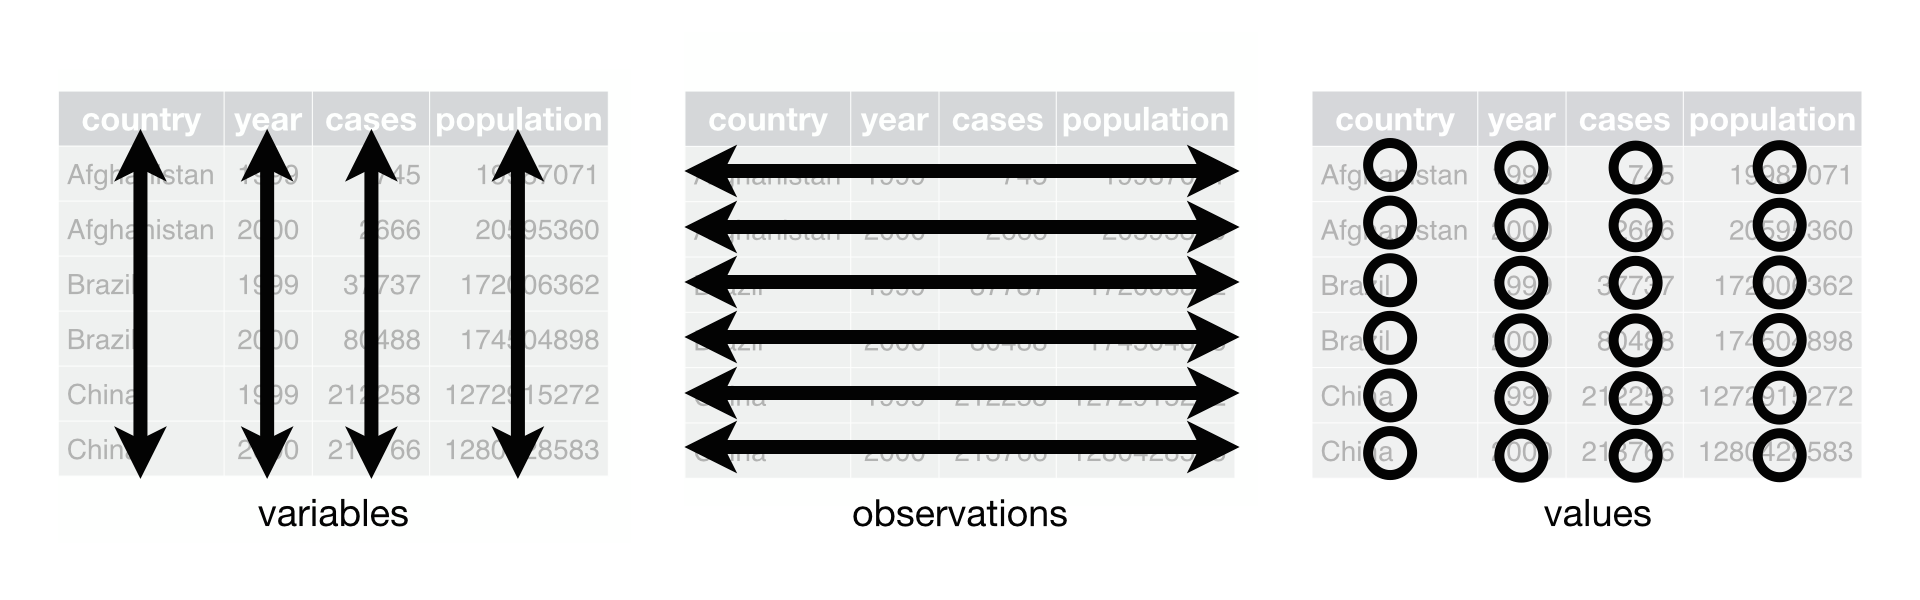
\includegraphics{fig/tidy-data-wickham.png} \emph{R for Data Science},
Wickham H and Grolemund G (\url{https://r4ds.had.co.nz/index.html}) ©
Wickham, Grolemund 2017 This image is licenced under
Attribution-NonCommercial-NoDerivs 3.0 United States (CC-BY-NC-ND 3.0
US)

In this section we will explore how these rules are linked to the
different data formats researchers are often interested in: ``wide'' and
``long''. This tutorial will help you efficiently transform your data
shape regardless of original format. First we will explore qualities of
the \texttt{interviews} data and how they relate to these different
types of data formats.

\subsubsection{Long and wide data
formats}\label{long-and-wide-data-formats}

In the \texttt{interviews} data, each row contains the values of
variables associated with each record collected (each interview in the
villages). It is stated that the \texttt{key\_ID} was ``added to provide
a unique Id for each observation'' and the \texttt{instanceID} ``does
this as well but it is not as convenient to use.''

Once we have established that \texttt{key\_ID} and \texttt{instanceID}
are both unique we can use either variable as an identifier
corresponding to the 131 interview records.

\begin{Shaded}
\begin{Highlighting}[]
\NormalTok{interviews }\SpecialCharTok{\%\textgreater{}\%} 
  \FunctionTok{select}\NormalTok{(key\_ID) }\SpecialCharTok{\%\textgreater{}\%} 
  \FunctionTok{distinct}\NormalTok{() }\SpecialCharTok{\%\textgreater{}\%} 
  \FunctionTok{count}\NormalTok{()}
\end{Highlighting}
\end{Shaded}

\begin{verbatim}
## # A tibble: 1 x 1
##       n
##   <int>
## 1   131
\end{verbatim}

\begin{Shaded}
\begin{Highlighting}[]
\NormalTok{interviews }\SpecialCharTok{\%\textgreater{}\%} 
  \FunctionTok{select}\NormalTok{(instanceID) }\SpecialCharTok{\%\textgreater{}\%} 
  \FunctionTok{distinct}\NormalTok{() }\SpecialCharTok{\%\textgreater{}\%} 
  \FunctionTok{count}\NormalTok{()}
\end{Highlighting}
\end{Shaded}

\begin{verbatim}
## # A tibble: 1 x 1
##       n
##   <int>
## 1   131
\end{verbatim}

As seen in the code below, for each interview date in each village no
\texttt{instanceID}s are the same. Thus, this format is what is called a
``long'' data format, where each observation occupies only one row in
the dataframe.

\begin{Shaded}
\begin{Highlighting}[]
\NormalTok{interviews }\SpecialCharTok{\%\textgreater{}\%}
  \FunctionTok{filter}\NormalTok{(village }\SpecialCharTok{==} \StringTok{"Chirodzo"}\NormalTok{) }\SpecialCharTok{\%\textgreater{}\%}
  \FunctionTok{select}\NormalTok{(key\_ID, village, interview\_date, instanceID) }\SpecialCharTok{\%\textgreater{}\%}
  \FunctionTok{sample\_n}\NormalTok{(}\AttributeTok{size =} \DecValTok{10}\NormalTok{)}
\end{Highlighting}
\end{Shaded}

\begin{verbatim}
## # A tibble: 10 x 4
##    key_ID village  interview_date      instanceID                               
##     <dbl> <chr>    <dttm>              <chr>                                    
##  1     60 Chirodzo 2016-11-16 00:00:00 uuid:85465caf-23e4-4283-bb72-a0ef30e30176
##  2    192 Chirodzo 2017-06-03 00:00:00 uuid:f94409a6-e461-4e4c-a6fb-0072d3d58b00
##  3     44 Chirodzo 2016-11-17 00:00:00 uuid:f9fadf44-d040-4fca-86c1-2835f79c4952
##  4     35 Chirodzo 2016-11-17 00:00:00 uuid:ff7496e7-984a-47d3-a8a1-13618b5683ce
##  5     37 Chirodzo 2016-11-17 00:00:00 uuid:408c6c93-d723-45ef-8dee-1b1bd3fe20cd
##  6      8 Chirodzo 2016-11-16 00:00:00 uuid:d6cee930-7be1-4fd9-88c0-82a08f90fb5a
##  7     49 Chirodzo 2016-11-16 00:00:00 uuid:2303ebc1-2b3c-475a-8916-b322ebf18440
##  8     36 Chirodzo 2016-11-17 00:00:00 uuid:c90eade0-1148-4a12-8c0e-6387a36f45b1
##  9     64 Chirodzo 2016-11-16 00:00:00 uuid:28cfd718-bf62-4d90-8100-55fafbe45d06
## 10     55 Chirodzo 2016-11-16 00:00:00 uuid:883c0433-9891-4121-bc63-744f082c1fa0
\end{verbatim}

We notice that the layout or format of the \texttt{interviews} data is
in a format that adheres to rules 1-3, where

\begin{itemize}
\tightlist
\item
  each column is a variable
\item
  each row is an observation
\item
  each value has its own cell
\end{itemize}

This is called a ``long'' data format. But, we notice that each column
represents a different variable. In the ``longest'' data format there
would only be three columns, one for the id variable, one for the
observed variable, and one for the observed value (of that variable).
This data format is quite unsightly and difficult to work with, so you
will rarely see it in use.

Alternatively, in a ``wide'' data format we see modifications to rule 1,
where each column no longer represents a single variable. Instead,
columns can represent different levels/values of a variable. For
instance, in some data you encounter the researchers may have chosen for
every survey date to be a different column.

These may sound like dramatically different data layouts, but there are
some tools that make transitions between these layouts much simpler than
you might think! The gif below shows how these two formats relate to
each other, and gives you an idea of how we can use R to shift from one
format to the other.

\includegraphics{fig/tidyr-pivot_wider_longer.gif} Long and wide
dataframe layouts mainly affect readability. You may find that visually
you may prefer the ``wide'' format, since you can see more of the data
on the screen. However, all of the R functions we have used thus far
expect for your data to be in a ``long'' data format. This is because
the long format is more machine readable and is closer to the formatting
of databases.

\subsubsection{Questions which warrant different data
formats}\label{questions-which-warrant-different-data-formats}

In interviews, each row contains the values of variables associated with
each record (the unit), values such as the village of the respondent,
the number of household members, or the type of wall their house had.
This format allows for us to make comparisons across individual surveys,
but what if we wanted to look at differences in households grouped by
different types of items owned?

To facilitate this comparison we would need to create a new table where
each row (the unit) was comprised of values of variables associated with
items owned (i.e., \texttt{items\_owned}). In practical terms this means
the values of the items in \texttt{items\_owned} (e.g.~bicycle, radio,
table, etc.) would become the names of column variables and the cells
would contain values of \texttt{TRUE} or \texttt{FALSE}, for whether
that household had that item.

Once we we've created this new table, we can explore the relationship
within and between villages. The key point here is that we are still
following a tidy data structure, but we have \textbf{reshaped} the data
according to the observations of interest.

Alternatively, if the interview dates were spread across multiple
columns, and we were interested in visualizing, within each village, how
irrigation conflicts have changed over time. This would require for the
interview date to be included in a single column rather than spread
across multiple columns. Thus, we would need to transform the column
names into values of a variable.

We can do both of these transformations with two \texttt{tidyr}
functions, \texttt{pivot\_wider()} and \texttt{pivot\_longer()}.

\subsection{Pivoting wider}\label{pivoting-wider}

\texttt{pivot\_wider()} takes three principal arguments:

\begin{enumerate}
\def\labelenumi{\arabic{enumi}.}
\tightlist
\item
  the data
\item
  the \emph{names\_from} column variable whose values will become new
  column names.
\item
  the \emph{values\_from} column variable whose values will fill the new
  column variables.
\end{enumerate}

Further arguments include \texttt{values\_fill} which, if set, fills in
missing values with the value provided.

Let's use \texttt{pivot\_wider()} to transform interviews to create new
columns for each item owned by a household. There are a couple of new
concepts in this transformation, so let's walk through it line by line.
First we create a new object (\texttt{interviews\_items\_owned}) based
on the \texttt{interviews} data frame.

\begin{Shaded}
\begin{Highlighting}[]
\NormalTok{interviews\_items\_owned }\OtherTok{\textless{}{-}}\NormalTok{ interviews }\SpecialCharTok{\%\textgreater{}\%}
\end{Highlighting}
\end{Shaded}

Then we will actually need to make our data frame longer, because we
have multiple items in a single cell. We will use a new function,
\texttt{separate\_longer\_delim()}, from the \textbf{\texttt{tidyr}}
package to separate the values of \texttt{items\_owned} based on the
presence of semi-colons (\texttt{;}). The values of this variable were
multiple items separated by semi-colons, so this action creates a row
for each item listed in a household's possession. Thus, we end up with a
long format version of the dataset, with multiple rows for each
respondent. For example, if a respondent has a television and a solar
panel, that respondent will now have two rows, one with ``television''
and the other with ``solar panel'' in the \texttt{items\_owned} column.

\begin{Shaded}
\begin{Highlighting}[]
\FunctionTok{separate\_longer\_delim}\NormalTok{(items\_owned, }\AttributeTok{delim =} \StringTok{";"}\NormalTok{) }\SpecialCharTok{\%\textgreater{}\%}
\end{Highlighting}
\end{Shaded}

After this transformation, you may notice that the \texttt{items\_owned}
column contains \texttt{NA} values. This is because some of the
respondents did not own any of the items in the interviewer's list. We
can use the \texttt{replace\_na()} function to change these \texttt{NA}
values to something more meaningful. The \texttt{replace\_na()} function
expects for you to give it a \texttt{list()} of columns that you would
like to replace the \texttt{NA} values in, and the value that you would
like to replace the \texttt{NA}s. This ends up looking like this:

\begin{Shaded}
\begin{Highlighting}[]
\FunctionTok{replace\_na}\NormalTok{(}\FunctionTok{list}\NormalTok{(}\AttributeTok{items\_owned =} \StringTok{"no\_listed\_items"}\NormalTok{)) }\SpecialCharTok{\%\textgreater{}\%}
\end{Highlighting}
\end{Shaded}

Next, we create a new variable named \texttt{items\_owned\_logical},
which has one value (\texttt{TRUE}) for every row. This makes sense,
since each item in every row was owned by that household. We are
constructing this variable so that when we spread the
\texttt{items\_owned} across multiple columns, we can fill the values of
those columns with logical values describing whether the household did
(\texttt{TRUE}) or did not (\texttt{FALSE}) own that particular item.

\begin{Shaded}
\begin{Highlighting}[]
\FunctionTok{mutate}\NormalTok{(}\AttributeTok{items\_owned\_logical =} \ConstantTok{TRUE}\NormalTok{) }\SpecialCharTok{\%\textgreater{}\%}
\end{Highlighting}
\end{Shaded}

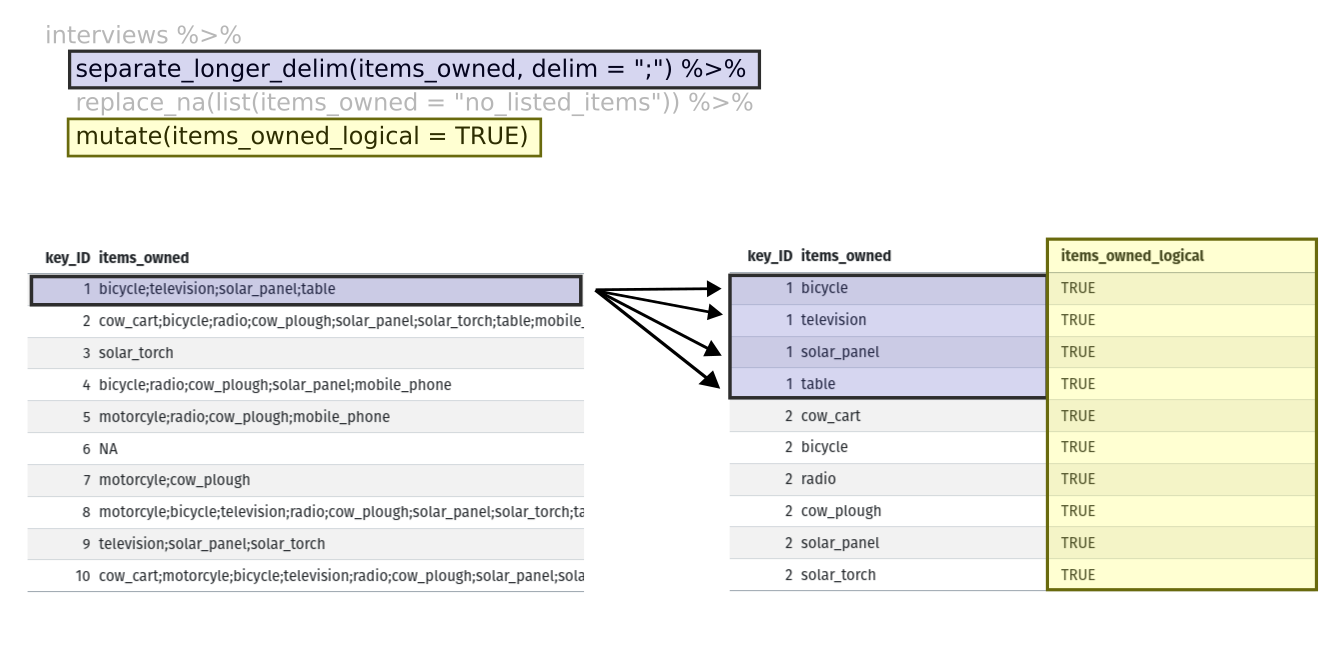
\includegraphics{fig/separate_longer.png}

At this point, we can also count the number of items owned by each
household, which is equivalent to the number of rows per
\texttt{key\_ID}. We can do this with a \texttt{group\_by()} and
\texttt{mutate()} pipeline that works similar to \texttt{group\_by()}
and \texttt{summarize()} discussed in the previous episode but instead
of creating a summary table, we will add another column called
\texttt{number\_items}. We use the \texttt{n()} function to count the
number of rows within each group. However, there is one difficulty we
need to take into account, namely those households that did not list any
items. These households now have \texttt{"no\_listed\_items"} under
\texttt{items\_owned}. We do not want to count this as an item but
instead show zero items. We can accomplish this using
\textbf{\texttt{dplyr}'s} \texttt{if\_else()} function that evaluates a
condition and returns one value if true and another if false. Here, if
the \texttt{items\_owned} column is \texttt{"no\_listed\_items"}, then a
0 is returned, otherwise, the number of rows per group is returned using
\texttt{n()}.

\begin{Shaded}
\begin{Highlighting}[]
\FunctionTok{group\_by}\NormalTok{(key\_ID) }\SpecialCharTok{\%\textgreater{}\%} 
  \FunctionTok{mutate}\NormalTok{(}\AttributeTok{number\_items =} \FunctionTok{if\_else}\NormalTok{(items\_owned }\SpecialCharTok{==} \StringTok{"no\_listed\_items"}\NormalTok{, }\DecValTok{0}\NormalTok{, }\FunctionTok{n}\NormalTok{())) }\SpecialCharTok{\%\textgreater{}\%} 
\end{Highlighting}
\end{Shaded}

Lastly, we use \texttt{pivot\_wider()} to switch from long format to
wide format. This creates a new column for each of the unique values in
the \texttt{items\_owned} column, and fills those columns with the
values of \texttt{items\_owned\_logical}. We also declare that for items
that are missing, we want to fill those cells with the value of
\texttt{FALSE} instead of \texttt{NA}.

\begin{Shaded}
\begin{Highlighting}[]
\FunctionTok{pivot\_wider}\NormalTok{(}\AttributeTok{names\_from =}\NormalTok{ items\_owned,}
            \AttributeTok{values\_from =}\NormalTok{ items\_owned\_logical,}
            \AttributeTok{values\_fill =} \FunctionTok{list}\NormalTok{(}\AttributeTok{items\_owned\_logical =} \ConstantTok{FALSE}\NormalTok{))}
\end{Highlighting}
\end{Shaded}

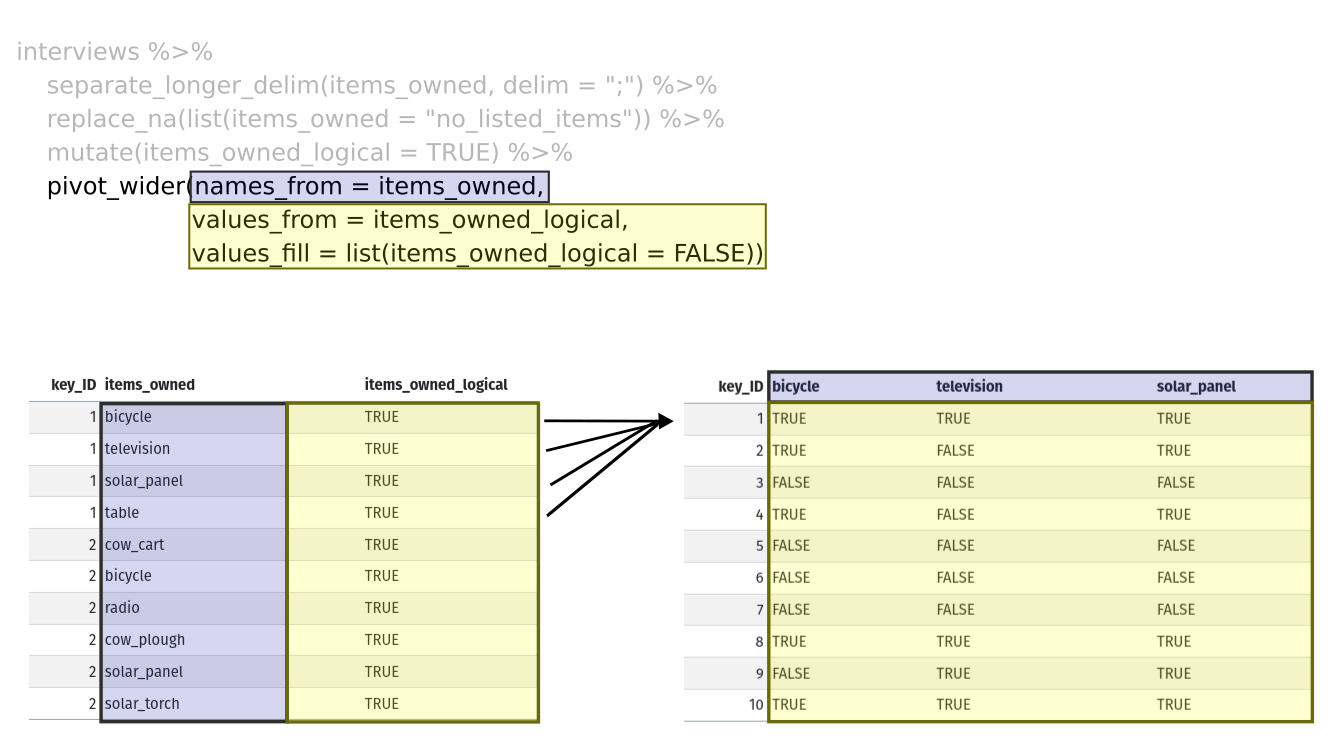
\includegraphics{fig/pivot_wider.png}

Combining the above steps, the chunk looks like this. Note that two new
columns are created within the same \texttt{mutate()} call.

\begin{Shaded}
\begin{Highlighting}[]
\NormalTok{interviews\_items\_owned }\OtherTok{\textless{}{-}}\NormalTok{ interviews }\SpecialCharTok{\%\textgreater{}\%}
  \FunctionTok{separate\_longer\_delim}\NormalTok{(items\_owned, }\AttributeTok{delim =} \StringTok{";"}\NormalTok{) }\SpecialCharTok{\%\textgreater{}\%}
  \FunctionTok{replace\_na}\NormalTok{(}\FunctionTok{list}\NormalTok{(}\AttributeTok{items\_owned =} \StringTok{"no\_listed\_items"}\NormalTok{)) }\SpecialCharTok{\%\textgreater{}\%}
  \FunctionTok{group\_by}\NormalTok{(key\_ID) }\SpecialCharTok{\%\textgreater{}\%}
  \FunctionTok{mutate}\NormalTok{(}\AttributeTok{items\_owned\_logical =} \ConstantTok{TRUE}\NormalTok{,}
         \AttributeTok{number\_items =} \FunctionTok{if\_else}\NormalTok{(items\_owned }\SpecialCharTok{==} \StringTok{"no\_listed\_items"}\NormalTok{, }\DecValTok{0}\NormalTok{, }\FunctionTok{n}\NormalTok{())) }\SpecialCharTok{\%\textgreater{}\%}
  \FunctionTok{pivot\_wider}\NormalTok{(}\AttributeTok{names\_from =}\NormalTok{ items\_owned,}
              \AttributeTok{values\_from =}\NormalTok{ items\_owned\_logical,}
              \AttributeTok{values\_fill =} \FunctionTok{list}\NormalTok{(}\AttributeTok{items\_owned\_logical =} \ConstantTok{FALSE}\NormalTok{))}
\end{Highlighting}
\end{Shaded}

View the \texttt{interviews\_items\_owned} data frame. It should have
\texttt{r\ nrow(interviews)} rows (the same number of rows you had
originally), but extra columns for each item. How many columns were
added? Notice that there is no longer a column titled
\texttt{items\_owned}. This is because there is a default parameter in
\texttt{pivot\_wider()} that drops the original column. The values that
were in that column have now become columns named \texttt{television},
\texttt{solar\_panel}, \texttt{table}, etc. You can use
\texttt{dim(interviews)} and \texttt{dim(interviews\_wide)} to see how
the number of columns has changed between the two datasets.

This format of the data allows us to do interesting things, like make a
table showing the number of respondents in each village who owned a
particular item:

\begin{Shaded}
\begin{Highlighting}[]
\NormalTok{interviews\_items\_owned }\SpecialCharTok{\%\textgreater{}\%}
  \FunctionTok{filter}\NormalTok{(bicycle) }\SpecialCharTok{\%\textgreater{}\%}
  \FunctionTok{group\_by}\NormalTok{(village) }\SpecialCharTok{\%\textgreater{}\%}
  \FunctionTok{count}\NormalTok{(bicycle)}
\end{Highlighting}
\end{Shaded}

\begin{verbatim}
## # A tibble: 3 x 3
## # Groups:   village [3]
##   village  bicycle     n
##   <chr>    <lgl>   <int>
## 1 Chirodzo TRUE       17
## 2 God      TRUE       23
## 3 Ruaca    TRUE       20
\end{verbatim}

Or below we calculate the average number of items from the list owned by
respondents in each village using the \texttt{number\_items} column we
created to count the items listed by each household.

\begin{Shaded}
\begin{Highlighting}[]
\NormalTok{interviews\_items\_owned }\SpecialCharTok{\%\textgreater{}\%}
    \FunctionTok{group\_by}\NormalTok{(village) }\SpecialCharTok{\%\textgreater{}\%}
    \FunctionTok{summarize}\NormalTok{(}\AttributeTok{mean\_items =} \FunctionTok{mean}\NormalTok{(number\_items))}
\end{Highlighting}
\end{Shaded}

\begin{verbatim}
## # A tibble: 3 x 2
##   village  mean_items
##   <chr>         <dbl>
## 1 Chirodzo       4.54
## 2 God            3.98
## 3 Ruaca          5.57
\end{verbatim}

\subsection{Exercise}\label{exercise}

We created \texttt{interviews\_items\_owned} by reshaping the data:
first longer and then wider. Replicate this process with the
\texttt{months\_lack\_food} column in the \texttt{interviews} dataframe.
Create a new dataframe with columns for each of the months filled with
logical vectors (\texttt{TRUE} or \texttt{FALSE}) and a summary column
called \texttt{number\_months\_lack\_food} that calculates the number of
months each household reported a lack of food.

Note that if the household did not lack food in the previous 12 months,
the value input was ``none''.

\subsection{Solution}\label{solution}

\begin{Shaded}
\begin{Highlighting}[]
\NormalTok{months\_lack\_food }\OtherTok{\textless{}{-}}\NormalTok{ interviews }\SpecialCharTok{\%\textgreater{}\%}
  \FunctionTok{separate\_longer\_delim}\NormalTok{(months\_lack\_food, }\AttributeTok{delim =} \StringTok{";"}\NormalTok{) }\SpecialCharTok{\%\textgreater{}\%}
  \FunctionTok{group\_by}\NormalTok{(key\_ID) }\SpecialCharTok{\%\textgreater{}\%}
  \FunctionTok{mutate}\NormalTok{(}\AttributeTok{months\_lack\_food\_logical =} \ConstantTok{TRUE}\NormalTok{,}
         \AttributeTok{number\_months\_lack\_food =} \FunctionTok{if\_else}\NormalTok{(months\_lack\_food }\SpecialCharTok{==} \StringTok{"none"}\NormalTok{, }\DecValTok{0}\NormalTok{, }\FunctionTok{n}\NormalTok{())) }\SpecialCharTok{\%\textgreater{}\%}
  \FunctionTok{pivot\_wider}\NormalTok{(}\AttributeTok{names\_from =}\NormalTok{ months\_lack\_food,}
              \AttributeTok{values\_from =}\NormalTok{ months\_lack\_food\_logical,}
              \AttributeTok{values\_fill =} \FunctionTok{list}\NormalTok{(}\AttributeTok{months\_lack\_food\_logical =} \ConstantTok{FALSE}\NormalTok{))}
\end{Highlighting}
\end{Shaded}

\subsection{Pivoting longer}\label{pivoting-longer}

The opposing situation could occur if we had been provided with data in
the form of \texttt{interviews\_wide}, where the items owned are column
names, but we wish to treat them as values of an \texttt{items\_owned}
variable instead.

In this situation we are gathering these columns turning them into a
pair of new variables. One variable includes the column names as values,
and the other variable contains the values in each cell previously
associated with the column names. We will do this in two steps to make
this process a bit clearer.

\texttt{pivot\_longer()} takes four principal arguments:

\begin{enumerate}
\def\labelenumi{\arabic{enumi}.}
\tightlist
\item
  the data
\item
  \emph{cols} are the names of the columns we use to fill the a new
  values variable (or to drop).
\item
  the \emph{names\_to} column variable we wish to create from the
  \emph{cols} provided.
\item
  the \emph{values\_to} column variable we wish to create and fill with
  values associated with the \emph{cols} provided.
\end{enumerate}

\begin{Shaded}
\begin{Highlighting}[]
\NormalTok{interviews\_long }\OtherTok{\textless{}{-}}\NormalTok{ interviews\_items\_owned }\SpecialCharTok{\%\textgreater{}\%}
  \FunctionTok{pivot\_longer}\NormalTok{(}\AttributeTok{cols =}\NormalTok{ bicycle}\SpecialCharTok{:}\NormalTok{car,}
               \AttributeTok{names\_to =} \StringTok{"items\_owned"}\NormalTok{,}
               \AttributeTok{values\_to =} \StringTok{"items\_owned\_logical"}\NormalTok{)}
\end{Highlighting}
\end{Shaded}

View both \texttt{interviews\_long} and
\texttt{interviews\_items\_owned} and compare their structure.

\subsection{Exercise}\label{exercise-1}

We created some summary tables on \texttt{interviews\_items\_owned}
using \texttt{count} and \texttt{summarise}. We can create the same
tables on \texttt{interviews\_long}, but this will require a different
process.

Make a table showing the number of respondents in each village who owned
a particular item, and include all items. The difference between this
format and the wide format is that you can now \texttt{count} all the
items using the \texttt{items\_owned} variable.

\subsection{Solution}\label{solution-1}

\begin{Shaded}
\begin{Highlighting}[]
\NormalTok{interviews\_long }\SpecialCharTok{\%\textgreater{}\%}
  \FunctionTok{filter}\NormalTok{(items\_owned\_logical) }\SpecialCharTok{\%\textgreater{}\%} 
  \FunctionTok{group\_by}\NormalTok{(village) }\SpecialCharTok{\%\textgreater{}\%} 
  \FunctionTok{count}\NormalTok{(items\_owned)}
\end{Highlighting}
\end{Shaded}

\begin{verbatim}
## # A tibble: 47 x 3
## # Groups:   village [3]
##    village  items_owned         n
##    <chr>    <chr>           <int>
##  1 Chirodzo bicycle            17
##  2 Chirodzo computer            2
##  3 Chirodzo cow_cart            6
##  4 Chirodzo cow_plough         20
##  5 Chirodzo electricity         1
##  6 Chirodzo fridge              1
##  7 Chirodzo lorry               1
##  8 Chirodzo mobile_phone       25
##  9 Chirodzo motorcyle          13
## 10 Chirodzo no_listed_items     3
## # i 37 more rows
\end{verbatim}

\subsection{Applying what we learned to clean our
data}\label{applying-what-we-learned-to-clean-our-data}

Now we have simultaneously learned about \texttt{pivot\_longer()} and
\texttt{pivot\_wider()}, and fixed a problem in the way our data is
structured. In this dataset, we have another column that stores multiple
values in a single cell. Some of the cells in the
\texttt{months\_lack\_food} column contain multiple months which, as
before, are separated by semi-colons (\texttt{;}).

To create a data frame where each of the columns contain only one value
per cell, we can repeat the steps we applied to \texttt{items\_owned}
and apply them to \texttt{months\_lack\_food}. Since we will be using
this data frame for the next episode, we will call it
\texttt{interviews\_plotting}.

\begin{Shaded}
\begin{Highlighting}[]
\DocumentationTok{\#\# Plotting data \#\#}
\NormalTok{interviews\_plotting }\OtherTok{\textless{}{-}}\NormalTok{ interviews }\SpecialCharTok{\%\textgreater{}\%}
  \DocumentationTok{\#\# pivot wider by items\_owned}
  \FunctionTok{separate\_longer\_delim}\NormalTok{(items\_owned, }\AttributeTok{delim =} \StringTok{";"}\NormalTok{) }\SpecialCharTok{\%\textgreater{}\%}
  \FunctionTok{replace\_na}\NormalTok{(}\FunctionTok{list}\NormalTok{(}\AttributeTok{items\_owned =} \StringTok{"no\_listed\_items"}\NormalTok{)) }\SpecialCharTok{\%\textgreater{}\%}
  \DocumentationTok{\#\# Use of grouped mutate to find number of rows}
  \FunctionTok{group\_by}\NormalTok{(key\_ID) }\SpecialCharTok{\%\textgreater{}\%} 
  \FunctionTok{mutate}\NormalTok{(}\AttributeTok{items\_owned\_logical =} \ConstantTok{TRUE}\NormalTok{,}
         \AttributeTok{number\_items =} \FunctionTok{if\_else}\NormalTok{(items\_owned }\SpecialCharTok{==} \StringTok{"no\_listed\_items"}\NormalTok{, }\DecValTok{0}\NormalTok{, }\FunctionTok{n}\NormalTok{())) }\SpecialCharTok{\%\textgreater{}\%} 
  \FunctionTok{pivot\_wider}\NormalTok{(}\AttributeTok{names\_from =}\NormalTok{ items\_owned,}
              \AttributeTok{values\_from =}\NormalTok{ items\_owned\_logical,}
              \AttributeTok{values\_fill =} \FunctionTok{list}\NormalTok{(}\AttributeTok{items\_owned\_logical =} \ConstantTok{FALSE}\NormalTok{)) }\SpecialCharTok{\%\textgreater{}\%} 
  \DocumentationTok{\#\# pivot wider by months\_lack\_food}
  \FunctionTok{separate\_longer\_delim}\NormalTok{(months\_lack\_food, }\AttributeTok{delim =} \StringTok{";"}\NormalTok{) }\SpecialCharTok{\%\textgreater{}\%}
  \FunctionTok{mutate}\NormalTok{(}\AttributeTok{months\_lack\_food\_logical =} \ConstantTok{TRUE}\NormalTok{,}
         \AttributeTok{number\_months\_lack\_food =} \FunctionTok{if\_else}\NormalTok{(months\_lack\_food }\SpecialCharTok{==} \StringTok{"none"}\NormalTok{, }\DecValTok{0}\NormalTok{, }\FunctionTok{n}\NormalTok{())) }\SpecialCharTok{\%\textgreater{}\%}
  \FunctionTok{pivot\_wider}\NormalTok{(}\AttributeTok{names\_from =}\NormalTok{ months\_lack\_food,}
              \AttributeTok{values\_from =}\NormalTok{ months\_lack\_food\_logical,}
              \AttributeTok{values\_fill =} \FunctionTok{list}\NormalTok{(}\AttributeTok{months\_lack\_food\_logical =} \ConstantTok{FALSE}\NormalTok{))}
\end{Highlighting}
\end{Shaded}

\subsection{Exporting data}\label{exporting-data}

Now that you have learned how to use \textbf{\texttt{dplyr}} and
\textbf{\texttt{tidyr}} to wrangle your raw data, you may want to export
these new datasets to share them with your collaborators or for archival
purposes.

Similar to the \texttt{read\_csv()} function used for reading CSV files
into R, there is a \texttt{write\_csv()} function that generates CSV
files from data frames.

Before using \texttt{write\_csv()}, we are going to create a new folder,
\texttt{data\_output}, in our working directory that will store this
generated dataset. We don't want to write generated datasets in the same
directory as our raw data. It's good practice to keep them separate. The
\texttt{data} folder should only contain the raw, unaltered data, and
should be left alone to make sure we don't delete or modify it. In
contrast, our script will generate the contents of the
\texttt{data\_output} directory, so even if the files it contains are
deleted, we can always re-generate them.

In preparation for our next lesson on plotting, we created a version of
the dataset where each of the columns includes only one data value. Now
we can save this data frame to our \texttt{data\_output} directory.

\begin{Shaded}
\begin{Highlighting}[]
\FunctionTok{write\_csv}\NormalTok{(interviews\_plotting, }\AttributeTok{file =} \StringTok{"data\_output/interviews\_plotting.csv"}\NormalTok{)}
\end{Highlighting}
\end{Shaded}

\begin{itemize}
\tightlist
\item
  Use the \texttt{tidyr} package to change the layout of data frames.
\item
  Use \texttt{pivot\_wider()} to go from long to wide format.
\item
  Use \texttt{pivot\_longer()} to go from wide to long format.
\end{itemize}

\end{document}
